% chapters/01_introduction.tex
% Regenerated 2026-07-12 via the regenerate-not-patch workflow (style_guide.md §6).
% Sonnet 5 authored four structurally divergent drafts from a bare-claims brief
% conditioned on Ch.4 rhythm spans; the "medical-lead" draft was selected, the
% sanctioned thesis bookend placed at the opening thesis position (once), and the
% chapter gated with voice_meter.py (per-file texture + cross-chapter n-grams vs the
% neighbor framing files). Diction pass: no figurative near-miss nouns.
% Framing locks (do not violate): spine = representation structure, BOTH lenses;
% arc = failure -> recovery -> detection; "guaranteed failure" is Ch.4-only; Ch.5
% diagnostic not impossibility; Ch.6 verb "matches-or-outperforms (in the mean)" /
% parity, never "beats"/"SOTA". No results numbers. Bookend to Ch.7.
\chapter{Introduction}
\label{ch:introduction}

A model trained on chest X-rays does not necessarily hesitate when shown a brain MRI. It may process the image as though it were another X-ray and return a confident diagnosis. That confidence is the problem: nothing in the output tells the user whether the model recognized something meaningful or merely chose among the labels it knows.

The brain-MRI example is an out-of-distribution (OOD) failure: the input differs
from the data on which the model was trained
\citep{hendrycks2016baseline,huang2020survey}. A related problem appears in
language models, which may invent plausible but nonexistent sources
\citep{li2023halueval,lin2021truthfulqa}. Although one problem concerns inputs and
the other outputs, both depend on whether the model's representation preserves
the information that distinguishes failure from ordinary behavior. If training
discards that information, no detector operating on the representation can
recover it; when the representation keeps it, a detector can read it out.

Information theory measures how much distinguishing information remains in a
representation \citep{shannon1948mathematical,cover1999elements}, while
representation geometry describes how that information is organized in feature
space. The three studies use both perspectives to trace a progression from
failure through recovery to detection (\Cref{fig:intro-spine}).

\begin{figure}[t]
  \centering
  \resizebox{\textwidth}{!}{%
  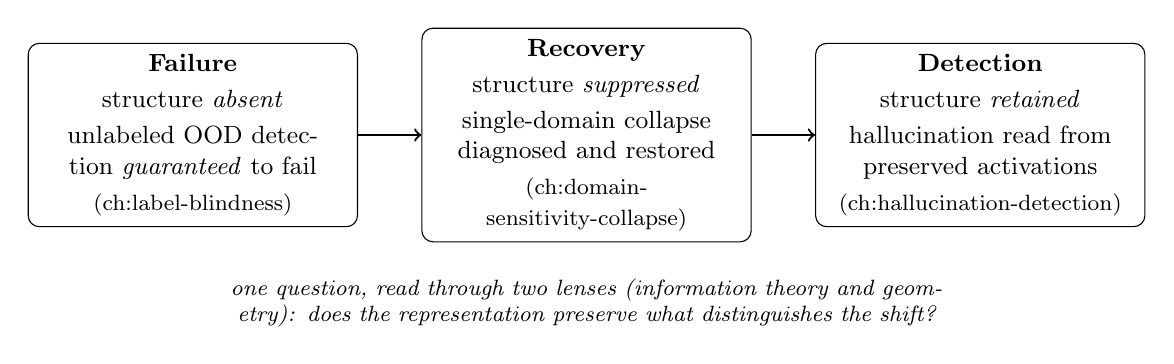
\begin{tikzpicture}[every node/.style={font=\small}]
    \tikzset{stage/.style={draw, rounded corners, text width=3.9cm, align=center,
      minimum height=2.2cm, inner sep=4pt}}
    \node[stage] (fail) at (0,0)
      {\textbf{Failure}\\[2pt] structure \emph{absent}\\[2pt]
       unlabeled OOD detection \emph{guaranteed} to fail\\[2pt]
       {\footnotesize(\Cref{ch:label-blindness})}};
    \node[stage] (rec) at (5,0)
      {\textbf{Recovery}\\[2pt] structure \emph{suppressed}\\[2pt]
       single-domain collapse diagnosed and restored\\[2pt]
       {\footnotesize(\Cref{ch:domain-sensitivity-collapse})}};
    \node[stage] (det) at (10,0)
      {\textbf{Detection}\\[2pt] structure \emph{retained}\\[2pt]
       hallucination read from preserved activations\\[2pt]
       {\footnotesize(\Cref{ch:hallucination-detection})}};
    \draw[->, thick] (fail) -- (rec);
    \draw[->, thick] (rec) -- (det);
    \node[font=\footnotesize\itshape, text width=11cm, align=center, anchor=north]
      at (5,-1.7)
      {one question, read through two lenses (information theory and geometry):
       does the representation preserve what distinguishes the shift?};
  \end{tikzpicture}%
  }
  \caption[The dissertation's spine]{The dissertation's spine. A single
  condition, whether the learned representation preserves the structure that
  distinguishes a shift, governs three reliability settings along one arc.}
  \label{fig:intro-spine}
\end{figure}

\section{Problem Statement and Motivation}
\label{sec:intro:problem}

Detection begins with the representation, not the scoring rule. Once a model has
been trained, a downstream detector can use only the distinctions preserved in
the model's features. The first question is therefore not which detector to
apply, but whether the training objective retained the information that detector
would need. The three studies examine different answers to this question.

\paragraph{Unlabeled OOD detection: structure absent.}
A self-supervised or unsupervised objective does not directly optimize for the
label distinction that defines an OOD task. When the features selected by that
objective are independent of the label-relevant features, the resulting
representation contains no usable signal about whether an example is
in-distribution or out-of-distribution. Under this condition, changing the
downstream detector cannot solve the problem. \Cref{ch:label-blindness}
formalizes this failure as label blindness. Its Adjacent OOD benchmark targets
the high-overlap regime in which the failure is most pronounced.

\paragraph{Single-domain OOD detection: structure suppressed.}
Supervised training preserves the features needed to separate known classes, but
training on a single domain can reduce sensitivity to directions that distinguish
one domain from another. \Cref{ch:domain-sensitivity-collapse} identifies this
effect as Domain-Sensitivity Collapse and shows how it weakens distance-based and
logit-based OOD detectors. Unlike label blindness, this is a diagnosis rather
than an impossibility result: the shift-sensitive structure can be strengthened.
Teacher-Guided Training restores that sensitivity by distilling knowledge from a
frozen multi-domain teacher without changing the model's inference-time cost.

\paragraph{Hallucination in large language models: structure retained.}
A language model's intermediate activations may preserve information about an
unsupported generation even when the final output does not reveal the failure.
\Cref{ch:hallucination-detection} asks whether the dependence between activations
at different layers provides enough signal for detection. It develops a
contrastive probe over cross-layer activation pairs to read out that signal from
a frozen model. Here the problem is not to recover information lost during
training, but to identify and use information that remains available internally.

\section{Research Objectives and Contributions}
\label{sec:intro:contributions}

This dissertation asks two related questions: when does a model's representation
make failure detection possible, and what can be done when the necessary
information is missing or suppressed? The three studies answer these questions
in different settings, while the fourth contribution brings their conclusions
into a common framework.

\begin{enumerate}
  \item \textbf{A limit on unlabeled OOD detection.}
  \Cref{ch:label-blindness} establishes a condition under which unlabeled OOD
  detection must fail. When a self-supervised objective selects features that
  are independent of the label-relevant distinction, the resulting
  representation provides no signal with which a downstream detector can
  distinguish in-distribution from out-of-distribution examples. We
  call this failure mode label blindness. The chapter presents the
  Adjacent OOD benchmark, which targets the high-overlap regime in which this
  limitation is most apparent. Full proofs appear in \Cref{app:proofs}.

  \item \textbf{A diagnosis and remedy for single-domain OOD detection.}
  \Cref{ch:domain-sensitivity-collapse} identifies Domain-Sensitivity Collapse
  (DSC), a process by which single-domain supervised training reduces variation
  along feature directions that distance- and logit-based detectors need. The
  resulting bounds diagnose why these detectors lose sensitivity without
  claiming that detection is impossible. The chapter then introduces
  Teacher-Guided Training (TGT), a training-time objective that distills a
  frozen multi-domain teacher to strengthen the suppressed directions without
  adding inference-time cost. Proofs appear in \Cref{app:dsc-proofs}.

  \item \textbf{A detector based on cross-layer language-model activations.}
  \Cref{ch:hallucination-detection} examines whether a language model retains
  information about hallucination in the dependence between its intermediate
  activations. A feasibility-by-trainability argument motivates a one-class
  contrastive probe over cross-layer activation pairs. The resulting detector
  matches or, in the mean, outperforms the strongest engineered probe in the
  comparison. An ablation also confirms a falsifiable prediction of the argument:
  symmetric contrastive supervision should fail. Proofs appear in
  \Cref{app:mi-hallucination-proofs}.

  \item \textbf{A common framework for detectability.}
  Taken together, the studies organize these problems around a single
  condition: whether the model's representation preserves the information
  needed to distinguish failure from ordinary behavior. Information theory
  describes whether that information remains, while feature-space geometry
  describes how it is organized and whether a detector can use it. Across the
  three studies, the relevant information is absent, suppressed but
  recoverable, or retained and available for readout.
\end{enumerate}

\section{Methodology and Approach}
\label{sec:intro:methodology}

The dissertation combines theoretical analysis with empirical evaluation. Each
study begins with the same object---a trained model's representation---and asks
what information it preserves about the distinction a detector must make.
\Cref{ch:background} develops the two perspectives used to answer that question:
information theory and feature-space geometry
\citep{shannon1948mathematical,cover1999elements,tishby2000information}.

The information-theoretic analysis treats a representation as a channel between
an input and the distinction of interest. In \Cref{ch:label-blindness}, this view
is used to determine when an unlabeled learning objective yields a representation
with no information needed for OOD detection. The resulting proof identifies a
specific condition under which no detector built on that representation can
distinguish in-distribution from out-of-distribution examples.
In \Cref{ch:hallucination-detection}, the same perspective is used in the opposite
direction: dependence between cross-layer activations provides a basis for asking
whether information about generation quality remains available for detection.

The geometric analysis in \Cref{ch:domain-sensitivity-collapse} asks how the
surviving information is arranged in feature space. In particular, it measures
whether single-domain training reduces variation along the directions that
distance- and logit-based OOD detectors use. The theoretical bounds describe
this loss of sensitivity, while Teacher-Guided Training tests whether guidance
from a multi-domain teacher can restore the affected geometry.

Empirical evaluations test each analysis in its corresponding regime:
high-overlap OOD detection, single-domain shift detection, and activation-based
hallucination detection. Controlled comparisons and ablations evaluate the
predicted mechanisms in each regime.

These methods support different conclusions: a conditional impossibility result
for label blindness, a diagnosis and empirically tested remedy for
Domain-Sensitivity Collapse, and a feasibility argument supported by parity with
the strongest engineered hallucination probe.

\section{Dissertation Organization}
\label{sec:intro:organization}

The dissertation proceeds from shared foundations to three studies and then to a
joint conclusion. Following this introduction, \Cref{ch:background} develops the
information-theoretic and geometric concepts used throughout the dissertation.
\Cref{ch:literature-review} then situates the research within prior work on OOD
detection, representation learning, and hallucination detection.

The next three chapters present the main studies. \Cref{ch:label-blindness}
establishes the label-blindness result and introduces the Adjacent OOD benchmark.
\Cref{ch:domain-sensitivity-collapse} analyzes Domain-Sensitivity Collapse and
develops Teacher-Guided Training as a remedy. \Cref{ch:hallucination-detection}
turns to language models and develops a contrastive detector based on cross-layer
activations. \Cref{ch:conclusion} brings the findings together, discusses the
limits of the common framework, and identifies directions for further research.

The complete proofs are collected in three appendices. \Cref{app:proofs}
supports the label-blindness result, \Cref{app:dsc-proofs} contains the
Domain-Sensitivity Collapse analysis, and \Cref{app:mi-hallucination-proofs}
provides the theory for hallucination detection.

\section{Significance}
\label{sec:intro:significance}

The central significance of this dissertation is that it separates detector
failure from representation failure. A benchmark can show that a particular
detector performs poorly, but it cannot determine whether another scoring rule
could succeed on the same representation. The label-blindness result answers
that deeper question under a stated independence condition: if the learning
objective preserves no information about the relevant distinction, changing the
downstream detector cannot help.

This distinction also determines what kind of intervention is appropriate. When
the information is absent, the representation or its training objective must
change. When it has been suppressed, as in Domain-Sensitivity Collapse, training
can restore the affected directions; Teacher-Guided Training does so without
adding inference-time cost. When the information remains internally available,
as the hallucination study investigates, a detector can be designed to read it
out from activations the model already computes.

The Adjacent OOD benchmark exposes a high-overlap regime that broad benchmarks
can obscure. Teacher-Guided Training addresses representation collapse in
narrow-domain models, while activation-based hallucination detection provides a
single-pass alternative to repeated sampling. Together, the studies establish
both limits on detection and interventions for cases in which useful information
can be restored or read out.
